\chapter{Implementación}

% \section{Introducción}

Este capítulo tratará sobre las herramientas utilizadas para la implementación y planificación, así como sobre los diferentes algoritmos utilizados para llevar a cabo la simulación.

\section{Herramientas utilizadas}

En el desarrollo del proyecto se utilizará \verb|git| para el control de versiones del proyecto y se almacenará en un repositorio de GitHub. Se hará uso de ramas 
% y \textit{Pull Requests} 
para implementar cada una de las historias de usuario, con el objetivo de seguir una metodología de trabajo similar a las que se realizan en metodologías ágiles.


% \bigskip

% En cuanto a la implementación de la aplicación, se utilizará C++ en las partes más críticas, en lugar de \textit{blueprints}. Para ello, se empleará Visual Studio como entorno de desarrollo.

\bigskip

% En cuanto a herramientas para la planificación, se hará uso de la herramienta \planApp para llevar un control de las Historias de Usuario que se realizan y pendientes en cada Sprint.
En lo que respecta a herramientas de planificación, se utilizará \planApp para llevar un control de las historias de usuario realizadas y pendientes en cada sprint.

% foto de \planApp
\begin{figure}[H]
    \centering
    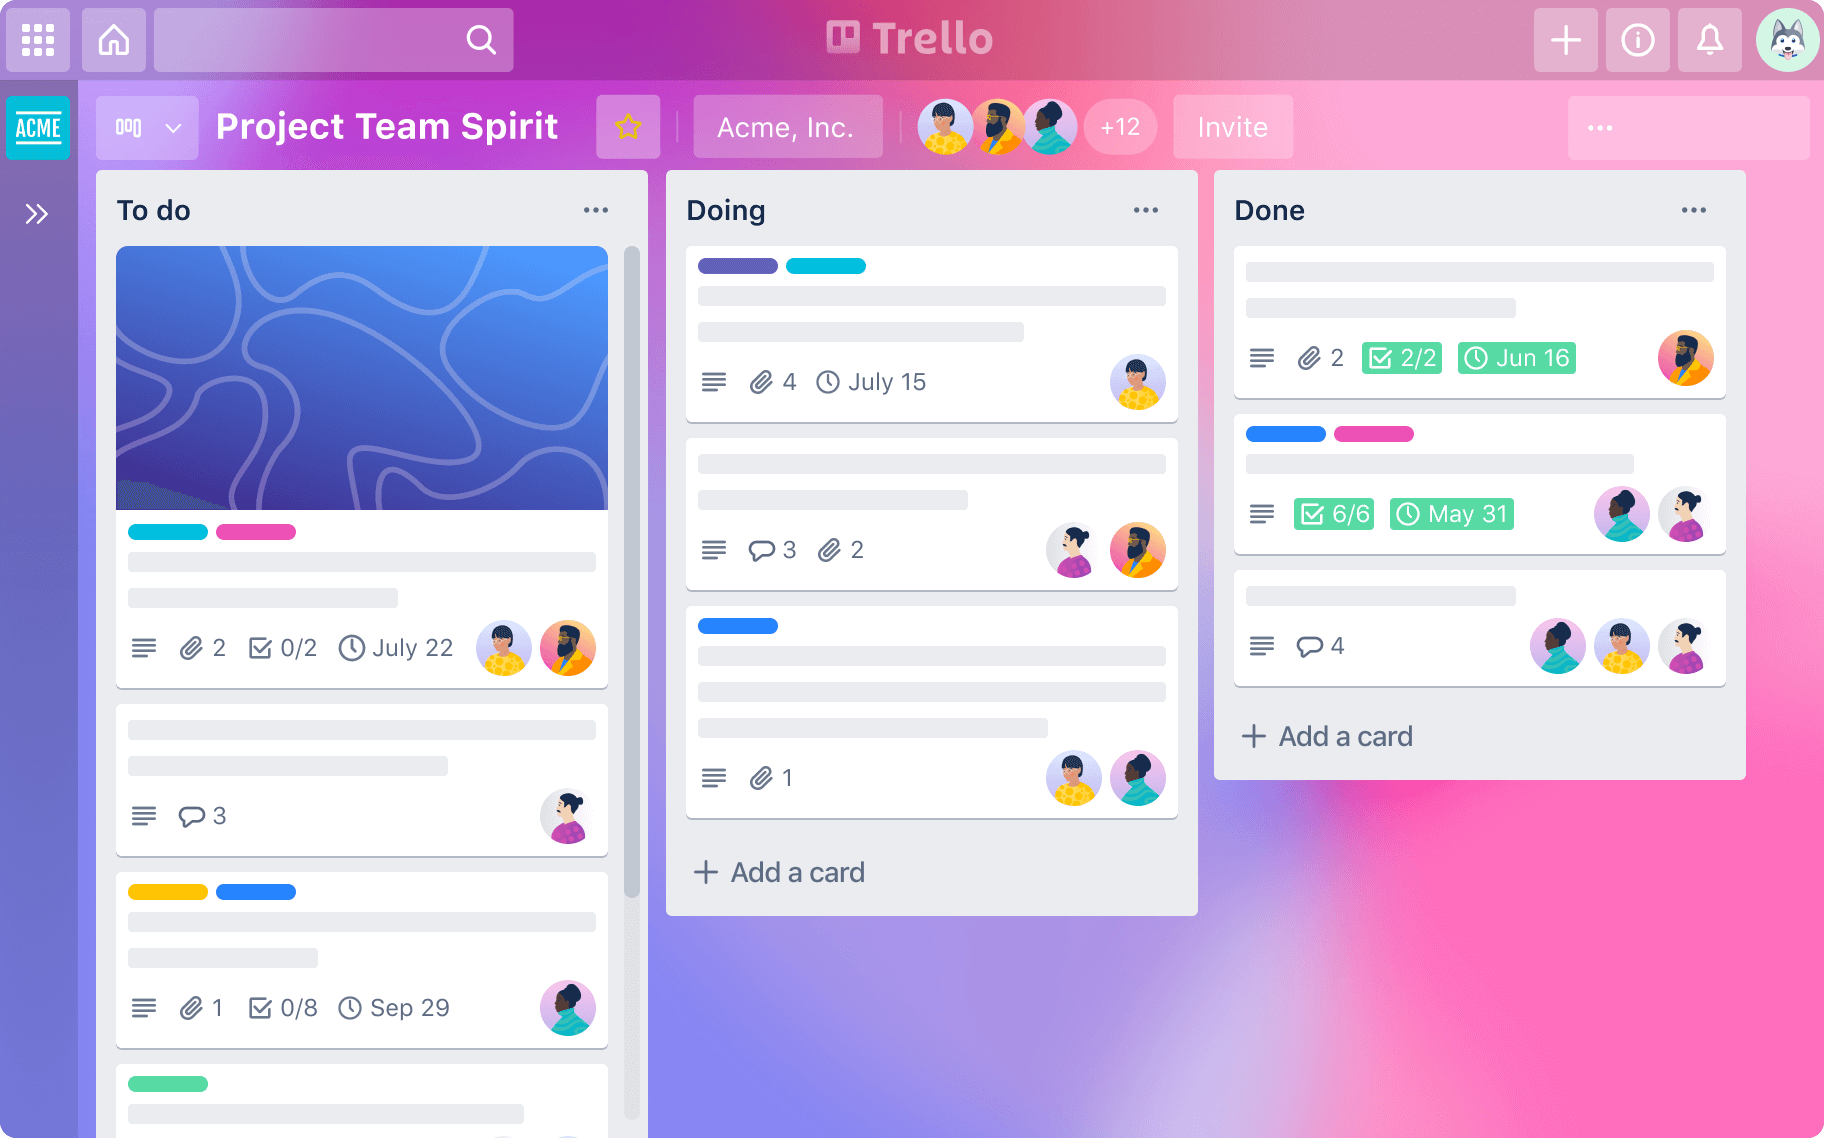
\includegraphics[width=0.75\textwidth]{imagenes/trello.png}
    \caption{Tablero de ejemplo de Trello\cite{tablero-trello}.}
\end{figure}

\section{Algoritmos utilizados}
En el control del volante de los vehículos, correspondiente a HU3 y realizada en el sprint 4, se ha utilizado un controlador PID, que consta de tres componentes: Proporcional, Integral y Derivativa. Utilizar un controlador de este tipo, en lugar de decidir el movimiento del volante directamente, presenta la ventaja de permitir un control más suave, con correcciones más realistas y con menos oscilaciones, siempre y cuando esté bien calibrado.

\bigskip

La calibración del PID se realiza modificando las constantes asociadas a cada componente. Existen diversos métodos como el de Ziegler-Nichols \cite{enwiki:1140258750}, que consiste en modificar solo la parte proporcional hasta que el coche comience a oscilar de manera estable, en ese momento se debe calcular la frecuencia a la que oscila para obtener las constantes finales mediante una fórmula. 

\bigskip

Dado que este método no me dio los resultados deseados, decidí implementar un algoritmo genético. Consiste en lanzar un conjunto de coches con valores aleatorios al principio, con el objetivo de que intenten llegar a la meta con el menor error posible. Aquellos con menos error, tienen más posibilidades de ser seleccionados para generaciones futuras. La selección se realiza lanzando una ruleta \cite{enwiki:1141636554}, la cual se divide según las probabilidades de cada coche. Una vez que se han elegido los coches que van a ser padres, se emparejan y se mezclan sus constantes para obtener dos hijos de cada pareja. Después, una de las componentes de algunos de los hijos se mutan y finalmente se sustituyen los coches no elegidos por los hijos, manteniendo también a los padres.

\bigskip

En cuanto al algoritmo de navegación, correspondiente a HU2, HU4 y HU5 e implementadas en los sprints 5 y 6, he utilizado \finalAlg para obtener la ruta más óptima. Este algoritmo debe ejecutarse en determinados momentos, ya que está pensado principalmente para entornos estáticos.

\bigskip

En lo que se refiere al cálculo de las posiciones de cada piloto, correspondientes a HU7 y HU8 e implementadas en el sprint 7, he utilizado una estructura de datos algo más compleja. Los vehículos almacenan la vuelta en la que están y el checkpoint; es decir, el sector del circuito en el que se encuentran. Con la información anterior, he creado un map que almacene como clave la vuelta y como valor otro map, que a su vez tiene como clave el checkpoint y como valor un array con todos los vehículos que se encuentran en ese estado. Para mostrarlo, solo hace falta iterar primero por aquellas claves mayores, ya que son los que más vueltas y más lejos del circuito están.

% foto de la estructura de datos
% \usepackage{multirow}

\begin{table}[H]
    \centering
    \begin{tblr}{
        cells = {c},
        row{1} = {Silver},
        cell{1}{2} = {c=2}{},
        cell{2}{1} = {r=4}{},
        cell{2}{2} = {Alto},
        cell{2}{3} = {Alto},
        cell{7}{1} = {r=2}{},
        cell{7}{2} = {Alto},
        cell{7}{3} = {Alto},
        vlines,
        hline{1-2,6-7,9} = {-}{},
        hline{3-5,8} = {2-3}{},
            }
        \textbf{Clave (vuelta actual)} & \textbf{Valor }                    &                \\
        0                              & \textbf{Clave (checkpoint actual)} & \textbf{Valor} \\
                                       & 0                                  & {[}c1]         \\
                                       & ...                                &                \\
                                       & i                                  & {[}c2, c3]     \\
        ...                            & ...                                & ...            \\
        i                              & \textbf{Clave (checkpoint actual)} & \textbf{Valor} \\
                                       & 3                                  & {[}c4]
    \end{tblr}
    \caption{Representación de la estructura de datos que almacena las posiciones de los pilotos durante la carrera.}
\end{table}

Para saber cuando lanzar la actualización de la lista de posiciones, cada coche calcula continuamente si el que está por delante de él sigue así, en caso contrario lanza el evento de actualización.

\bigskip

En cuanto a la actualización del contador de vueltas, correspondiente a HU9 y realizado en el sprint 8, he hecho que todos los coches cuando acaben una vuelta intenten actualizarlo, en caso de que la vuelta actual sea mayor o igual, no se actualiza. De esta forma, es más fácil llevar un control más preciso de las vueltas.